%% compile with pdflatex or xelatex
\documentclass[11pt,a4paper]{article}
\usepackage[fontset=ubuntu]{ctex}
\usepackage{homework}

\title{Homework 1}
\duedate{Mar 3, 2020}


\studentname{Charles Shen}
\studentid{2017013569}

\usepackage{tikz}
\usetikzlibrary{automata,shapes,positioning,arrows}

%% logical symbols
% \land     /\
% \lor      \/
% \lnor     (negation)
% \to       ->
% \lequiv   <->
% \models   |=
\newcommand{\lequiv}{\leftrightarrow}

\begin{document}
	
	\maketitle
	
	\textit{Read the instructions below carefully before you start working on the assignment:}
	\begin{itemize}
		\item Please typeset your answers in the attached \LaTeX~source file, compile it to a PDF,
		and finally hand the PDF to Tsinghua Web Learning \emph{before the due date}.
		\item Make sure you fill in your \emph{name} and \emph{Tsinghua ID},
		and replace all ``\texttt{TODO}''s with your solutions.
		\item Any kind of dishonesty is \emph{strictly prohibited} in the full semester.
		If you refer to any material that is not provided by us, you \emph{must cite} it.
	\end{itemize}
	
	%% problem begins
	
	\problem{True of False}
	
	Are the following statements true or false? If false, provide a counterexample.
	
	\subproblem Given an arbitrary propositional logic formula, the problem of deciding its validity is decidable.
	
	\begin{solution}
		True.
	\end{solution}
	
	\subproblem If a propositional logic formula is not valid, then it is unsatisfiable.
	
	\begin{solution}
		False.\\
		Consider F=P, when P is False, F is False, F is not valid. But when P is True, F is True, F is satisfiable.
		
	\end{solution}
	
	\subproblem Every NNF is also a CNF.
	
	\begin{solution}
		False.\\
		$(\lnot P \land \lnot Q)\lor R$ is a NNF, but not a CNF.
	\end{solution}
	
	\subproblem A propositional logic formula $\varphi$ is satisfiable if and only if for every interpretation $I$,
	$I \models \varphi$.
	
	\begin{solution}
		False.\\
		$\phi = P$ is satisfiable, since there exists $I = {P \mapsto true}, I \models \phi$.But there also exists $I = {P \mapsto false}, I \not\models \phi$.
	\end{solution}
	
	\subproblem If clause $C$ is a unit under an interpretation $I$, then $I \not\models C$.
	
	\begin{solution}
		False.\\
		Consider $C = P \lor Q, I = \{P \mapsto true, Q \mapsto undef\}. \\
		C' = P, l = Q, C = C' \lor l, I \not \models C'$, C is unit under I, but $I \not\models C$ is not right in such case. 
	\end{solution}
	
	\newpage
	\problem{Normal Forms}
	
	\subproblem Convert the following formula into NNF and then DNF:
	$$\lnot(\lnot(P \land Q) \to \lnot R)$$
	
	\begin{solution}
		1.$\lnot((P \land Q) \lor \lnot R)$\\
		2.$\lnot (P \land Q) \land R$\\
		3.$(\lnot P \lor \lnot Q) \land R$, Now it is a NNF\\
		4.$(\lnot P \land R)\lor (\lnot Q \land R)$,Now it is a DNF.
	\end{solution}
	
	\subproblem Convert the following formula into CNF with and without Tseitin's transformation:
	$$(P \to (\lnot Q \land R)) \land (P \to \lnot Q)$$
	
	\begin{solution}
		No Tseitin:\\
		1.$(\lnot P \lor (\lnot Q \land R))\land(\lnot P \lor \lnot Q)$\\
		2.$(\lnot P \lor \lnot Q)\land (\lnot P \lor R) \land (\lnot P \lor \lnot Q)$\\
		Tseitin:\\
		$F1 = T1 \lequiv \lnot Q \land R \\
		= (\lnot T1 \lor \lnot Q)\land (\lnot T1 \lor R) \land (Q \lor \lnot R \lor T1)$\\
		$F2 = T2 \lequiv P \to T1 \\
		= (\not T2 \lor \lnot P \lor T1) \land (P \lor T2) \land (\lnot T1 \lor T2) $\\
		$F3 = T3 \lequiv P \to \lnot Q \\
		= (\lnot T3 \lor \lnot P \lor \lnot Q) \land (P \lor T3) \land (Q \lor T3)
		$\\
		$F4 = T4 \lequiv T2 \land T3 \\
		= (\lnot T4 \lor T2) \land (\lnot T4 \lor T3) \land (\lnot T2 \lor \lnot T3 \lor T4)
		$\\
		$F = T4 \land F1 \land F2 \land F3 \land F4$
		
	\end{solution}
	
	\newpage
	\problem{Validity \& Satisfiability}
	
	\subproblem Consider the following formula:
	$$(P \to (Q \to R)) \to (\lnot R \to (\lnot Q \to \lnot P))$$
	Is it valid? If not, provide a falsifying interpretation.
	Moreover, is it satisfiable? If so, provide a satisfying interpretation.
	
	\begin{solution}
		Not Valid, consider $ I = \{ P |\mapsto true, Q |\mapsto false, R |\mapsto false \}$\\
		Satisfiable, consider $I= \{ P |\mapsto true, Q |\mapsto true, R |\mapsto true \}$
	\end{solution}
	
	\subproblem Show the validity of the following formula using the semantic argument method:
	$$\lnot(P \land Q) \lequiv (\lnot P \lor \lnot Q)$$
	
	\begin{solution}
		$
		1.I \nvDash \lnot(P \land Q) \lequiv (\lnot P \lor \lnot Q)\\
		2.I \models (P \land Q) \land (\lnot P \lor \lnot Q) (1,\lequiv, caseA)\\
		3.I \models \lnot(P \land Q) \land (P \land Q) (1,\lequiv, caseB)\\
		4.I \models P \land Q (2, \land, caseA)\\
		5.I \models \lnot P \lor \lnot Q (2, \land, caseA)\\
		6.I \nvDash P \land Q (5, \lnot, caseA) \\
		$For case A, 4 and 6 reach a contradiction.\\$
		7.I \models \lnot (P \land Q) (3, \land , caseB)\\
		8.I \models (P \land Q) (3, \land, caseB)\\
		$For case A, 7 and 8 reach a contradiction.\\
		Since all the branches have reached contradiction, the formula given above is valid.
		
	\end{solution}
	
	\subproblem Show the satisfiability of the following formula by resolution:
	$$(\lnot P \lor \lnot Q) \land (\lnot P \lor R) \land (Q \lor \lnot R)$$
	Then, give a general form of all satisfying interpretations.
	
	\begin{solution}
		Round 1:\\
		$F1 = \lnot P \lor \lnot Q \\
		F2 = \lnot P \lor R \\
		F3 = Q \lor \lnot R \\
		F' = \empty \\
		F = \{F1, F2, F3 \} \\
		$
		Round 2:\\
		$
		F4 = \lnot P \lor \lnot R (1\&3)\\
		F5 = \lnot P \lor Q (2\&3) \\
		F' = \{F4,F5\}\\
		F = \{F1,F2,F3,F4,F5\}\\
		$
		Round 3:\\
		$
		F6 = \lnot P (1\&5)\\
		F' = \{F4,F5,F6\}\\
		F = \{F1,F2,F3,F4,F5,F6\}\\
		$
		Round 4:\\
		$
		F' = \{F4,F5,F6\}\\
		F = \{F1,F2,F3,F4,F5,F6\}\\
		F' \subseteq F\\
		$
		Therefore, the formula is satisfiable.\\
		The general form is $\{P \mapsto false, Q \mapsto true\} or \{P \mapsto false, R \mapsto false\}.$
		\end{solution}
		
		\newpage
		\problem{Modeling}
		
		A \emph{nondeterministic finite automaton} (NFA) is given by a 5-tuple $(Q, \Sigma, \delta, I, F)$, where:
		\begin{itemize}
		\item $Q$ is a finite set of states
		\item $\Sigma$ is a finite alphabet
		\item $\delta: Q \times \Sigma \times 2^Q$ is a transition function
		\item $I \subseteq Q$ is a set of initial states
		\item $F \subseteq Q$ is a set of final (accepting) states
		\end{itemize}
		
		An NFA accepts a finite word (or, a char sequence) $w = [c_0, \ldots, c_n]$, where $c_i \in \Sigma$,
		if and only if there is a sequence of states $q_0, \ldots, q_n$, with $q_i \in Q$, such that:
		\begin{itemize}
		\item $q_0 \in I$
		\item For all $i \in \{1, \ldots, n\}$, $q_i \in \delta(q_{i-1}, w_i)$
		\item $q_n \in F$
		\end{itemize}
		
		\subproblem Given an NFA $M=(Q, \Sigma, \delta, I, F)$ and a fixed input string $w$,
		describe how to construct a propositional formula that is satisfiable if and only if $M$ accepts $w$.
		
		\hint{Consider defining propositional variables that correspond to the initial states, final states,
			transition function, and alphabet symbols in $w$. Then think about ``unwinding'' the NFA on $w$.
			Do you need to define additional variables? How can you encode the fact that $w$ is accepted?}
		
		\begin{solution}
		为了避免空产生式带来的不利影响,我们首先把NFA转化为DFA进行处理。\\
		假设w长度为n,转化的DFA有m个状态:$q_{0},q_{1}...q_{m-1}$,其状态转移为$\sigma$。输入串w在DFA中的路径为$q_{s_{0}},q_{s_{1}}...q_{s_{n}}$\\
		定义两种类型的文字:$S_{i,j}(0 \leq i \leq n; q_{j} \in Q)$代表已经输入i个字符后,状态为$q_{j}$,特别的,i为0代表初态为$q_{j}$。$C_{i,j,k}(q_{i}, q_{k} \in Q; j \in \Sigma)$代表当前状态为$q_{i}$时,输入j,状态变为$q_{k}$。\\
		设计成这样:要保证所有的文字满足以下几点,才成立:\\
		1.初态正确:当且仅当$q_{j}$为初态,$S_{0,j}$为真。这个规则是为了保证输入前状态在初态。\\
		2.终态正确:当且仅当$q_{j}$为终态,$S_{n,j}$为真。这个规则是为了保证输入w完毕后状态可接受。\\
		3.转换正确:对于任意的$1 \leq t \leq n; q_{i},q_{k} \in Q, j \in \Sigma$,当仅当$\sigma(q_{i},j)=q_{k}$,有$S_{t-1,i} \land S_{t,k} \land C_{i,j,k}$为真。这个规则是为了保证每一步转换严格按照自动机规则进行。\\
		如果w可以被自动机接受,那么不会产生矛盾,这个式子可满足。\\
		相反,如果w不可被自动机接受,那么规则3要求终态对应的$S_{n,q_{s_{n}}}$为真,规则2要求终态对应的$S_{n,q_{s_{n}}}$为假,矛盾,这个式子不可满足。
		$F = \bigwedge_{q_{i} \in I}S_{0,i} \\
		\land \bigwedge_{q_{i} \notin I}\lnot(S_{0,i}) \\
		\land \bigwedge_{q_{i} \in F}S_{n,i} \\
		\land \bigwedge_{q_{i} \notin F}\lnot(S_{n,i}) \\
		\land \bigwedge_{1 \leq t \leq n;q_{s_{t-1}}, q_{s_{t}} \in Q; \sigma(q_{s_{t-1}},w_{t})=q_{s_{t}}}(S_{t - 1,s_{t-1}} \land C_{s_{t-1}, w_{t}, s_{t}} \land S_{t, s_{t}}) \\
		$
		\end{solution}
		
		\subproblem Demonstrate your encoding on the NFA shown in \cref{fig:nfa}.
		
		\begin{figure}[ht]
		\begin{minipage}{.45\textwidth}
		\centering
		\begin{align*}
		Q &= \{q_0, q_1, q_2, q_3\} \\
		\Sigma &= \{0, 1\} \\
		\delta &= \{\!\begin{aligned}[t]
		& (q_0, 0) \mapsto q_0, \\
		& (q_0, 1) \mapsto q_0, \\
		& (q_0, 0) \mapsto q_1, \\
		& (q_0, 1) \mapsto q_2, \\
		& (q_1, 0) \mapsto q_3, \\
		& (q_2, 1) \mapsto q_3, \\
		& (q_3, 0) \mapsto q_3, \\
		& (q_3, 1) \mapsto q_3 \}
		\end{aligned} \\
		I &= \{q_0\} \\
		F &= \{q_3\}
		\end{align*}
		\end{minipage}
		% mid
		\begin{minipage}{.48\textwidth}
		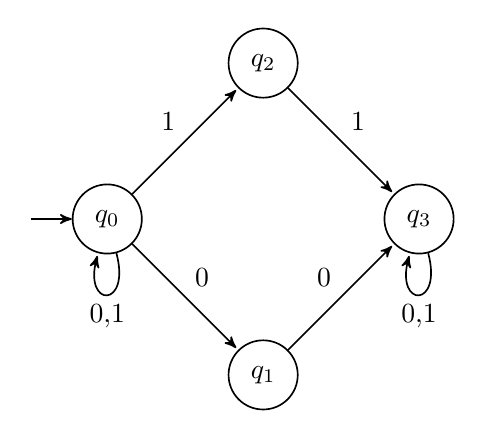
\begin{tikzpicture}[->,>=stealth',shorten >=1pt,auto,node distance=2.8cm,semithick]
		
		\node[state] (q0)                     {$q_0$};
		\node[state] (q2) [above right of=q0] {$q_2$};
		\node[state] (q1) [below right of=q0] {$q_1$};
		\node[state] (q3) [below right of=q2] {$q_3$};
		
		\draw[<-] (q0) -- ++(-1cm,0);
		
		\path (q0) edge [loop below] node {0,1} (q0)
		edge              node {0}   (q1)
		edge              node {1}   (q2)
		(q1) edge              node {0}   (q3)
		(q2) edge              node {1}   (q3)
		(q3) edge [loop below] node {0,1} (q3);
		\end{tikzpicture}
		\end{minipage}
		\caption{An NFA.}
		\label{fig:nfa}
		\end{figure}
		
		\begin{solution}
		1.将这个NFA转化为DFA,如下:\\
		\begin{figure}[ht]
		\begin{minipage}{.45\textwidth}
		\centering
		\begin{align*}
		Q &= \{q_0, q_1, q_2, q_3,q_4\} \\
		\Sigma &= \{0, 1\} \\
		\delta &= \{\!\begin{aligned}[t]
		& (q_0, 0) \mapsto q_0, \\
		& (q_0, 1) \mapsto q_2, \\
		& (q_1, 0) \mapsto q_3, \\
		& (q_1, 1) \mapsto q_2, \\
		& (q_2, 0) \mapsto q_1, \\
		& (q_2, 1) \mapsto q_4, \\
		& (q_3, 0) \mapsto q_3, \\
		& (q_3, 1) \mapsto q_4 \\
		& (q_4, 0) \mapsto q_3 \\
		& (q_4, 1) \mapsto q_4 \}
		\end{aligned} \\
		I &= \{q_0\} \\
		F &= \{q_3,q_4\}
		\end{align*}
		\end{minipage}
		% mid
		\begin{minipage}{.48\textwidth}
		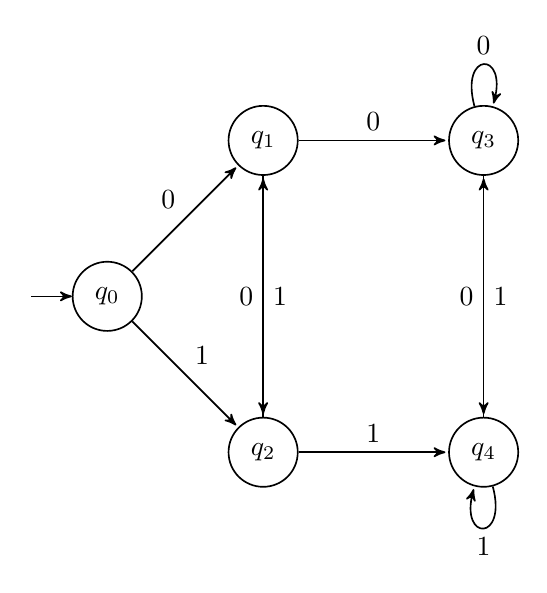
\begin{tikzpicture}[->,>=stealth',shorten >=1pt,auto,node distance=2.8cm,semithick]
		
		\node[state] (q0)                     {$q_0$};
		\node[state] (q1) [above right of=q0] {$q_1$};
		\node[state] (q2) [below right of=q0] {$q_2$};
		\node[state] (q3) [right of=q1] {$q_3$};
		\node[state] (q4) [right of=q2] {$q_4$};
		\draw[<-] (q0) -- ++(-1cm,0);
		
		\path 
		(q0) edge              node {0}   (q1)
		edge              node {1}   (q2)
		(q1) edge              node {0}   (q3)
		edge              node {1}   (q2)
		(q2) edge              node {0}   (q1)
		edge              node {1}   (q4)
		(q3) edge [loop above] node {0}   (q3)
		edge              node {1}   (q4)
		(q4) edge [loop below] node {1}   (q4)
		edge              node {0}   (q3)
		;
		\end{tikzpicture}
		\end{minipage}
		\caption{The DFA according to the problem.}
		\label{fig:nfa}
		\end{figure}
		令w = 00, 那么路径变为 $q_{0},q_{1},q_{3}$,式子变为\\
		$S_{00}\land \lnot S_{01} \land \lnot S_{02}\land \lnot S_{03}\land \lnot S_{04} \land S_{11} \land C_{001} \land C_{103} \land S_{23} \land S_{24} \\land \lnot S_{20}\land \lnot S_{21}\land \lnot S_{22}$
		\end{solution}
		
		%% problem ends
		
		\end{document}